%!TEX root = /Users/daniel/Documents/thesis/thesis.tex
\chapter{Motivation}

\section{\LaTeX}

Wenn es um das Verfassen wissenschaftlicher Texte geht, ist für viele \LaTeX\ die erste Wahl. Anders als bei einem \ac{WYSIWYG}-Editor kümmert man sich nicht um das Layout, um Abstände und Schriftgrößen sondern um die Semantik des Geschriebenen. Man zeichnet die Kapitel, Abschnitte, Formeln usw. aus, eher wie in \ac{HTML} als in MS-Word. Der Vorteil liegt auf der Hand. Inhalt und Präsentation sind klar getrennt, was zur Folge hat, dass man nicht vom Wesentlichen abgelenkt wird, wenn man an Texten und Formeln arbeitet, und dass das Aussehen des Dokuments zentral in der Präambel definiert wird.

\LaTeX~hat jedoch auch seine Nachteile. Gerade Anfänger haben es aufgrund der flachen Lernkurve schwer. Da man \LaTeX~in der Regel im Quelltext bearbeitet, also jeden Befehl von Hand schreibt, muss man sich unheimlich viel merken. Das beginnt bei einfachen Befehlen wie \texttt{\textbackslash chapter}, deren Name sich geradezu aufdrängt, aber wenn es darum geht Mathematische Formeln wie $$\Gamma \left( x \right) = \int\limits_0^\infty  {s^{x - 1} e^{ - s} ds}$$ in das Dokument zu bringen, wird es schon schwieriger.

Dass man ein $\Gamma$ mit dem Befehl \texttt{\textbackslash Gamma} bekommt ist noch zu erahnen. Um $\infty$ zu bekommen hätte man auch \texttt{\textbackslash infinity} statt \texttt{\textbackslash infty} versuchen können und hätte bloß einen Fehler geerntet, aber bei Befehlen wie \texttt{\textbackslash leftrightsquigarrow} ($\leftrightsquigarrow$) hört jede Intuition auf. Es ist also offensichtlich, dass es einigen Raum für unterstützende Maßnahmen bei der Erstellung von \LaTeX-Dokumenten gibt. Das gilt insbesondere für mathematische Formeln in denen viele unterschiedliche Symbole vorkommen können.

\section{Die optimale Eingabemethode}
\label{sec:optimal}

Überlegt man sich die natürlichste oder zumindest gewohnteste Art Text oder Mathematik zu notieren, so kommt man unweigerlich auf Stift und Papier. Während bei Texten die Eingabe über eine Computertastatur durchaus schneller sein kann als das Schreiben mit einem Stift, ist spätestens bei Formeln klar, dass hier der Stift im Vorteil ist\footnote{Allgemein ist die Eingabe mit einer Tastatur bei kleinen Alphabeten schneller, jedoch bei großen Alphabeten nicht mehr praktikabel \cite{Tappert:1990p10302}.}. Es können beliebige Formen, Zeichen und Symbole in beliebige räumliche Beziehung gebracht werden. Nichts liegt also näher, als diese Eingabeform in die digitale Welt übertragen zu wollen.

Als Eingabegerät bietet sich also ein Grafiktablett an. Ein entsprechender \LaTeX-Editor würde eine Fläche zur Verfügung stellen, auf die einfach geschrieben und skizziert wird. Die Kurven und Linien würden dann vom Editor in Text, Tabellen, Formeln und Diagramme überführt -- alles genau wie vom Benutzer erwartet. Dies ist eine Vision, die es seit 1995 gibt \cite{Meyer:1995p10480}. Leider sind wir 15 Jahre später immer noch nicht so weit.

Alleine der Bereich der mathematischen Formelerkennung ist noch nicht auf einem Level, auf dem man die verfügbaren Lösungen als gut bezeichnen könnte. Es gibt kaum kommerzielle Lösungen und eine Hand voll experimentelle Tools. Nur wenige davon haben überhaupt \LaTeX~oder Textsatz allgemein als Fokus. Andere gehen eher in Richtung interaktive Mathematik oder sogar \ac{CAS}.

\subsection{Infty Editor}

Ein Beispiel für einen Editor, der beim Textsatz helfen soll ist die kostenlose Software \href{http://www.inftyproject.org}{InftyEditor} \cite{Suzuki:2003p786}. Sie ermöglicht die Eingabe von Formeln in einem interessanten Mix aus \ac{WYSIWYG}-Editor und \LaTeX-Autovervollständigung mit Vorschau (siehe Abb.~\ref{fig:inftyeditor-autocomplete}). 

InftyEditor hat außerdem eine Funktion handgeschriebene Formeln zu erkennen. Dazu öffnet man das InftyHandWriting Input Pad und fängt an zu zeichnen. Einfache Formeln werden damit auch noch recht sicher erkannt, aber sobald die Komplexität der Formel steigt und vor allem sobald man Symbole braucht, die die Software gar nicht kennt, wird die Benutzung zum Frusterlebnis. Abb.~\ref{fig:inftyeditor} zeigt das InftyHandwriting Input Pad.

\begin{figure}
  \begin{center}
    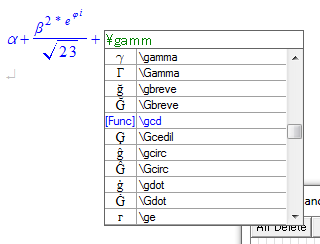
\includegraphics[width=\textwidth]{figures/inftyeditor-autocomplete.png}
  \end{center}
  \caption{InftyEditor Autovervollständigung}
  \label{fig:inftyeditor-autocomplete}
\end{figure}

\begin{figure}
  \begin{center}
    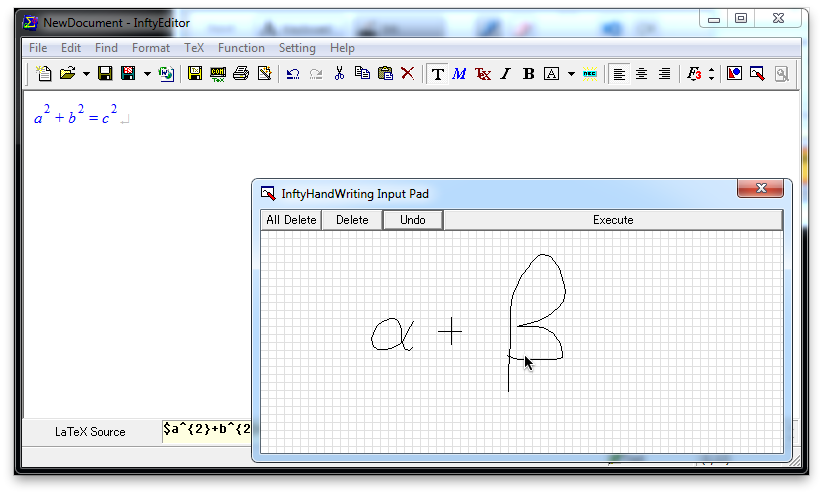
\includegraphics[width=\textwidth]{figures/inftyeditor.png}
  \end{center}
  \caption{InftyEditor}
  \label{fig:inftyeditor}
\end{figure}


\subsection{Freehand Formula Entry System}

http://research.cs.queensu.ca/drl/ffes/

Lorem Ipsum\dots \TODO Paper ansehen

\subsection{Natural Log}

\TODO ist ein Witz\dots 

\subsection{JMathNotes}

\TODO ansehen + Paper gibts nicht

\subsection{Microsoft Math}

Microsoft Math ist ein kommerzielles Produkt, das aber nicht für den Textsatz gedacht ist, sondern eher mit einem programmierbaren Taschenrechner zu vergleichen ist. Die Eingabe erfolgt entweder über die Tatstatur (Abb. \ref{fig:ms-math-keyboard}) oder über Handschrifterkennung (Abb. \ref{fig:ms-math-ink}) und die Handschrifterkennung macht zwar einen solideren Eindruck als bei den vorgenannten Produkten, ist aber auch noch nicht der Weissheit letzter Schluss. Abb. \ref{fig:ms-math-ink} zeigt einen Versuch die Gammafunktion zu erkennen und der Erfolg ist zweifelhaft.

Ist die Formel dann auf welche Weise auch immer eingegeben, so kann dann damit einiges angestellt werden, was aber nicht im Interesse dieser Arbeit liegt und darum auch nicht näher beschrieben wird.

\begin{figure}
  \begin{center}
    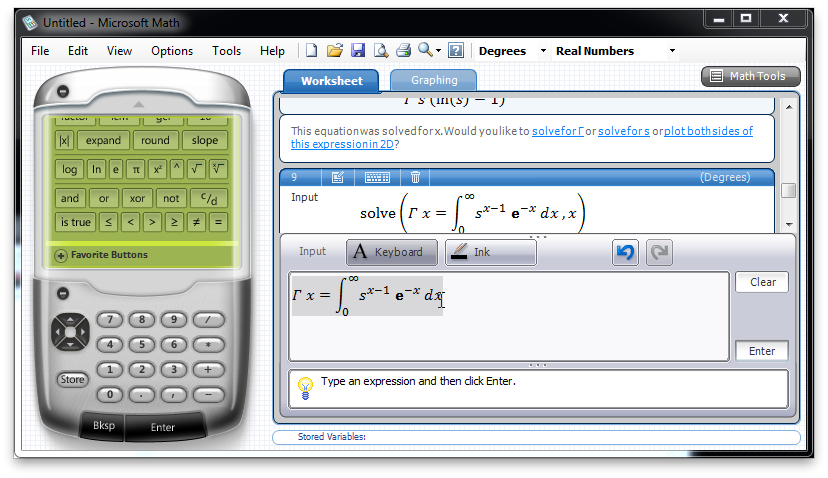
\includegraphics[width=\textwidth]{figures/ms-math-keyboard.png}
  \end{center}
  \caption{Microsoft Math 3.0 Tastatureingabe}
  \label{fig:ms-math-keyboard}
\end{figure}

\begin{figure}
  \begin{center}
    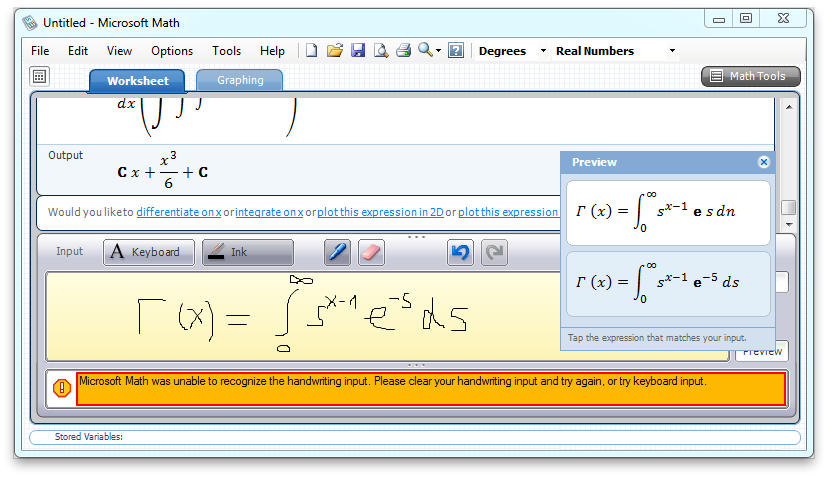
\includegraphics[width=\textwidth]{figures/ms-math-ink.png}
  \end{center}
  \caption{Microsoft Math 3.0 Handschrifterkennung}
  \label{fig:ms-math-ink}
\end{figure}


\subsection{MathJournal}

Lorem Ipsum\dots \TODO Paper ansehen

\subsection{MathBrush}

Lorem Ipsum\dots \TODO Paper ansehen

\TODO Sollte noch erwähnen, dass ich nur LaTeX machen will und kein ComputerAlgebra..

\subsection{WebMath}

\TODO \cite{Vuong:2010p10279}

\section{Was ist so schwierig?}

Das Problem teilt sich dabei in drei Teile auf. Das erste ist die Segmentierung der mathematischen Formel, bei der einzelne Symbole isoliert werden müssen. Als zweites müssen die einzelnen Symbole richtig erkannt werden. Schließlich müssen die Symbole über ihre räumliche Position in eine logische Beziehung zueinander gebracht werden. Die in diesen Schritten gewonnenen Erkenntnisse können natürlich die Entscheidung in den jeweils anderen beeinflussen, indem man die Semantik einer Interpretation in der Erkennung mit einfließen lässt. Das Problem ist also sehr komplex. \cite{Tapia:2007p9160} ist ein aktueller Übersichtsartikel, der die Problematik genauer beleuchtet.

\TODO Auf interaktive Fehlerbehebung eingehen? MathBrush hat sowas. Und ich hab sowas auch schon in den Artikeln gesehen


\section{Suche nach Alternativen}
\label{sec:alternativen}

\TODO Detexify ist trotzdem nützlich, selbst wenn man sowas wie Infty oder ffes benutzt um bei der Korrenktur einzende Symbole einzufügen die vorher mit Detexify gesucht werden können.

Die optimale Eingabemethode ist also (noch) nicht praktikabel. Um ganze Formeln zuverlässig zu erkennen haben wir noch nicht die optimalen Algorithmen gefunden. Eine Alternative ist, dem Computer nur einen Teil der Erkennung zu übertragen. Ein Beispiel hierfür ist \href{http://jequation.sourceforge.net/}{JEquation}. In diesem Programm wird dem Benutzer vorgegeben, wo der zu malen hat, damit die Struktur der Formel richtig erkannt wird. Es bleibt also die Aufgabe die einzelnen Symbole zu erkennen. \TODO Bild? Und welche Kritik habe ich an diesem Ansatz?

Es gibt natürlich auch Ansätze, die ohne jede Form von Mustererkennung auskommen. Hier ist \href{http://lyx.org}{Lyx} ein Beispiel. Lyx ist ein \ac{WYSIWYM}-Editor. Er funktioniert also ähnlich wie ein \ac{WYSIWYG}-Editor wie MS-Word. Dabei arbeitet man nicht direkt mit \LaTeX-Befehlen sondern hat einen graphischen Editor in dem man jedoch die Textabschnitte semantisch auszeichnet, statt den Schriftstil manuell vorzugeben. Für Mathematische Formeln enthält Lyx einen Formeleditor, der ähnlich dem funktioniert, was aus Office-Paketen wie MS-Word bekannt ist. Um Symbole einzufügen hat man einerseits die Möglichkeit direkt \LaTeX-Befehle (mit Auto-Vervollständigung) direkt einzugeben, oder das gesuchte Symbol aus mehreren Symboltabellen auszuwählen und per Klick einzufügen. Die erste der beiden Möglichkeiten setzt natürlich wieder voraus, dass der Author den Namen des Befehls kennt. Die zweite Methode hat den Nachteil, dass die Symboltabellen schnell unübersichtlich werden, wenn sie zu umfangreich sind. Es lässt sich also nur ein kleiner Teil der verfügbaren Symbole unterbringen, ohne den Nutzen zu kompromittieren.

\section{Ein pragmatischer Ansatz} % (fold)
\label{sec:pragmatisch}

Viele Benutzer fühlen sich aber durchaus wohl damit ihre Dokumente direkt im Quelltext zu bearbeiten. Texteditoren wie Vim, Emacs etc. erfreuen sich großer Beliebtheit zum erstellen von Dokumenten. (\TODO Wie belege ich das? Internet?) Ich selbst ziehe den Texteditor Vim trotz umfangreicher Recherchen in diesem Bereich jedem spezialisierten \LaTeX-Editor vor. Die Frage ist also, wie ein pragmatisches Werkzeug aussieht, dass einem typischen Anwender die Arbeit an seinem Dokument insbesondere die Eingabe von mathematischen Formeln erleichtert ohne dessen Arbeitsweise komplett umzukrempeln.

Ein Problem, das jeder Anwender egal ob Einsteiger oder Fortgeschrittener einmal hat, ist, dass er den Befehl für ein Symbol nicht weiss. Vielleicht hat er ihn noch nie gebraucht, oder er ist ihm entfallen. Das Symbol ist auch nicht in den Symboltabellen in seinem \LaTeX-Editor (falls er nicht sowieso einen Texteditor verwendet). Also muss er ein Buch oder die "`Comprehensive \LaTeX\ Symbol List"'~\cite{Pakin:2009p2664} wälzen, um das gewünschte Symbol zu finden. Das geht bei der großen Anzahl an Symbolen~\footnote{\cite{Pakin:2009p2664} listet 4947 unterschiedliche Symbole auf.} nicht besonders schnell. Genau hier könnte ein pragmatisches Werkzeug ansetzen und auf einem Mittelweg zwischen den in \ref{sec:alternativen} vorgestellten Werkzeugen eine Lösung für dieses Problem anbieten.

Das Werkzeug müsste also Symbolsuche bieten, durch die sehr schnell der Befehl zum gesuchten Symbol gefunden werden kann. Der Benutzer kann sein Dokument im Editor seiner Wahl bearbeiten und im Bedarfsfall das Suchwerkzeug aufrufen, um schnell wieder an die eigentliche Arbeit, das Verfassen des Dokuments, zu gehen. Um ein solches Werkzeug wird es im folgenden gehen.

% section ein_pragmatischer_ansatz (end)
